\subsection{Visión por Computadora}
La visión por computadora (VC) es una subdisciplina de la inteligencia artificial que busca dotar a las máquinas de la capacidad de interpretar y comprender imágenes del mundo real. En la visión computacional se busca describir el mundo que vemos en una o más imágenes y reconstruir sus características, como la forma, la iluminación y las distribuciones de color. 
Esto es algo que el ser humano puede hacer de manera natural pero que dentro de un algoritmo de visión por computador se vuelve complejo y propenso a errores (\cite{szeliski2010computer}). Asimismo, como menciona (\cite{klette2010computer}), esta disciplina tiene como objetivo utilizar cámaras para analizar o comprender escenas en el mundo real. 
Por otro lado, según (\cite{sucar2008vision}), la visión computacional es el estudio de los procesos de reconocer y localizar objetos usando el procesamiento de imágenes de tal forma que se logre un mayor entendimiento de estos. Por lo tanto, la visión computacional busca el entendimiento, análisis y descripción de lo visto en imágenes del mundo real para poder, posteriormente, aplicar lo comprendido hacia algún objetivo. 

Por otro lado, de acuerdo con (\cite{szeliski2010computer}), el preprocesamiento de imágenes es el primer paso en la mayoría de las aplicaciones de visión computacional. Esto se realiza para procesar la imagen y convertirla en un resultado que sea adecuado para realizar mayor análisis.

Adicionalmente, la visión computacional estudia problemas metodológicos y algorítmicos, así como temas relacionados con la implementación de soluciones relacionadas. Por ejemplo, esta hace posible analizar la distancia de un edificio hacia una cámara, detectar si un vehículo está dentro de su carril, reconocer personas o contar la cantidad de personas en una escena (\cite{klette2014concise}). Por lo tanto, la visión computacional es muy amplia y abarca distintos campos de aplicación y estudio, entre estos campos se encuentran los siguientes (\cite{szeliski2010computer}): 

\begin{itemize}
    \item Reconocimiento de Caracteres (OCR): por ejemplo, aplicado en el reconocimiento 
de códigos escritos a mano o placas de automóviles.
    \item Imágenes Médicas: aplicado en el análisis de imágenes médicas preoperatorias e 
intraoperatorias.
    \item Construcción de modelos 3D a partir de imágenes
    \item Reconocimiento de objetos en retail: el reconocimiento de productos en las colas de pago.  
    \item Seguridad vehicular: aplicado en la detección de obstáculos en las calles como los peatones.
    \item Videovigilancia: se puede aplicar para el monitoreo del comportamiento de los clientes y análisis de tráfico en los retail.
\end{itemize}

Luego, en el siglo XXI, nacieron nuevas áreas de investigación como el campo de fotografía computacional, esto ayudó a realizar mejoras en imágenes digitales mediante algoritmos como, por ejemplo, las imágenes de alto rango dinámico (HDR). Adicionalmente, surgieron las técnicas basadas en descriptores de características para detección de objetos (Feature-based recognition). 

Finalmente, empezaron a investigarse nuevos campos basados en el aprendizaje automático (machine learning) (\cite{szeliski2010computer}). El aprendizaje automático posteriormente dio paso al aprendizaje profundo o deep learning. 
En la actualidad, las técnicas de deep learning han tomado mayor importancia dentro de la visión computacional. En los últimos años, se ha demostrado que los métodos de deep learning superan a las técnicas de aprendizaje automático de última generación en varios campos, siendo la visión por computadora uno de los casos más destacados. Los modelos de deep learning aplicados a visión computacional incluyen las redes neuronales convolucionales, las máquinas de Boltzmann (DBM) y redes de creencia profunda (DBN) (\cite{voulodimos2018deep}). 

El deep learning ha impulsado considerablemente el desarrollo de la visión computacional en aplicaciones como la detección de objetos, el seguimiento de movimiento, la detección de poses, entre otros. 

En el caso de las redes neuronales convolucionales, estas han sido muy útiles en aplicaciones de visión por computadora, tales como reconocimiento facial, detección de objetos, robótica y vehículos autónomos (\cite{voulodimos2018deep}). 

\subsubsection{Técnicas de Visión por Computadora}
La visión por computadora ha evolucionado rápidamente gracias a los avances en el aprendizaje profundo y el aumento en la capacidad de procesamiento de datos. Las técnicas más destacadas son diseñada para abordar desafíos específicos en el análisis de imágenes.

\paragraph{1. Redes Neuronales Convolucionales (CNN):}
Se utilizan redes neuronales convolucionales (CNN) para clasificar y detectar objetos en imagenes. En el caso de las redes neuronales convolucionales, estas han sido muy útiles en aplicaciones de visión por computadora, tales como reconocimiento facial, detección de objetos, robótica y vehículos autónomos (\cite{voulodimos2018deep}). 

Las  redes neuronales convolucionales (CNN) son fundamentales en visión por computadora y son especialmente efectivas en tareas de clasificación y reconocimiento de imágenes debido a su capacidad para capturar patrones locales y características espaciales en los datos visuales (\cite{gupta2023cnn}). Las CNN funcionan mediante capas de convolución que extraen características específicas, como bordes o texturas, y capas de agrupamiento (pooling) que reducen la dimensionalidad de los datos, manteniendo la información esencial. Modelos como AlexNet y VGGNet han demostrado ser especialmente efectivos al aumentar la profundidad de la red, lo que permite captar características más complejas en imágenes (\cite{zhang2024deep, ieee2023alexnet}).

\paragraph{2. Transformers Vision:}
Es un algoritmo de segmentación basados en aprendizaje profundo. Han ganado popularidad en la visión por computadora gracias a su capacidad para procesar grandes cantidades de datos sin perder detalles contextuales. A diferencia de las CNN, que son locales, los transformers de visión utilizan autoatención para analizar relaciones en toda la imagen de manera global. Esto los convierte en una herramienta valiosa para tareas como la segmentación semántica y la detección de objetos en escenas complejas, permitiendo una mejor precisión en entornos dinámicos.

\paragraph{3. Arquitecturas de Redes Profundas: Inception, ResNet y Xception}
Además de las CNN y los transformers, arquitecturas como Inception, ResNet y Xception han introducido innovaciones significativas en el campo de la visión por computadora. Inception, por ejemplo, utiliza una combinación de convoluciones de diferentes tamaños para capturar múltiples escalas de características en una sola capa, mejorando la eficiencia sin sacrificar la precisión. ResNet, por otro lado, resuelve el problema de la desaparición de gradientes al permitir conexiones de salto (skip connections), lo que facilita la construcción de redes extremadamente profundas sin pérdida de rendimiento (IEEE, 2023). Xception, una evolución de Inception, reemplaza las convoluciones tradicionales con convoluciones separables en profundidad, optimizando el procesamiento de datos y logrando un mejor rendimiento en grandes conjuntos de datos visuales (\cite{zhang2024deep}).

Finalmente, como se puede observar, el campo de la visión computacional es bien amplio 
e incluye aplicaciones en diversos sectores: industriales, de consumo masivo, retail, 
automóviles, entre otros. Es un campo con áreas de investigación y de aplicación muy diversas. Asimismo, sus algoritmos han ido evolucionando considerablemente en el tiempo, pero manteniendo la premisa básica de buscar reconstruir y comprender las características del mundo real a partir de imágenes. La investigación se centra en una parte de este universo, específicamente en su aplicación para la detección y verificación facial. 


\subsection{Inteligencia Artificial}
La inteligencia según (\cite{dezhic2018intelligence}) es “La capacidad de percibir o inferir información, y de retenerla como conocimiento que debe aplicarse a conductas adaptativas dentro de un entorno o contexto”. Además, la inteligencia artificial es una manera de entender la inteligencia e integrarla en el software y dispositivos de hardware (\cite{maheshwari2018ai}). 

A diferencia de las innovaciones más especializadas, la inteligencia artificial se está convirtiendo en una verdadera tecnología de propósito general. Es decir, se está convirtiendo en una utilidad no muy diferente a la electricidad, que probablemente se extenderá todas las industrias y sectores de nuestra economía, y en casi todos los aspectos de la ciencia, la sociedad y la cultura (\cite{ford2018ai}).

La inteligencia no es propiamente una tecnología. Es más bien, una parte de las Ciencias de la Computación, que se enfoca en permitir que, en cualquier momento, una computadora perciba y responda a su entorno (\cite{norman2018computing}). 

Esta organización de la inteligencia artificial se realiza en torno a tres categorías 
principales: 

\begin{itemize}
    \item Técnicas de inteligencia artificial: modos avanzados de modelos estadísticos y matemáticos, como la lógica difusa, el aprendizaje automático y los sistemas expertos, que se utilizan en el cálculo de tareas que normalmente realizan los humanos. Se pueden utilizar para implementar diversas funciones de la inteligencia artificial.
    \item Aplicaciones funcionales de la inteligencia artificial: funciones como el habla o la visión por computadora.
    \item Campos de aplicación de la inteligencia artificial: son los diferentes campos, áreas o disciplinas donde las aplicaciones de la inteligencia artificial se emplean (como en el transporte, la agricultura o las ciencias médicas).
\end{itemize}

La Inteligencia Artificial o IA es unos de los campos más nuevos en la ciencia, no solo intenta entender, sino que va más allá y construye entidades inteligentes. Actualmente, abarca muchos subcampos que van de lo general a lo específico como matemáticas, salud, escribir poesías, conducir un automóvil, entre otros. (\cite{russel2010ai}). Además, según (\cite{utnfrbam2021}) La inteligencia artificial se define como la capacidad de las máquinas para llevar a cabo actividades que generalmente demandan inteligencia humana, como programar, diagnosticar enfermedades, resolver problemas matemáticos complejos, analizar circuitos electrónicos, y comprender y generar lenguaje humano. La IA se basa en la creación de sistemas que pueden exhibir comportamientos inteligentes o que puedan ser considerados inteligentes si fueran realizados por humanos.

Básicamente, la IA es una tecnología desarrollada capaz de imitar las funciones cognitivas del ser humano. Dentro de ella diferenciamos 3 tipos fundamentales:
\begin{itemize}
    \item Estrecha o débil: Metodología de aprendizaje que se focaliza en una tarea única. La mayor parte de los algoritmos de IA se desarrolla en la salud con IA estrecha. Por ejemplo, en el diagnostico de enfermedades.
    \item General: Modelo que equipara la función de IA a las capacidades humanas. Actualmente enfocada a la gestión de la incertidumbre; por ejemplo, a la prediccion de modelos predictivos de la salud.
    \item Super IA: Campo futurible en el que la IA superaría la capacidad humana en todos los campos. Se trata de la IA mostrada en muchas superproducciones como la verdadera IA, que no es más que ciencia ficción en la sociedad actual por ejemplo films orientados a la IA.
\end{itemize}

Finalmente, las técnicas de inteligencia artificial (\cite{heredia2015ai}), son de gran importancia hoy en día para mejorar los sistemas de información, donde los algoritmos son capaces de sustituir personas en el análisis de información (\cite{massa2018ai}), realizando tareas como en el procesamiento de volúmenes de datos que al ser analizados (\cite{bobadilla2019data}), logramos  pasar de tener información a transformarla en conocimiento (\cite{garcia2018knowledge}) permitiendo a los administradores del negocio  mejorar los resultado en la toma de decisiones.

\subsection{YOLO 5}
Hoy en día, uno de los grupos de algoritmos de detección de objetos más populares es YOLO, que se puede utilizar en tareas de detección de objetos en tiempo real y cuyos algoritmos de grupo permiten obtener resultados prometedores en diferentes áreas. Por supuesto, existen muchas versiones del algoritmo YOLO, desde la primera versión original de YOLO hasta YOLOv8, YOLO-NAS y YOLO con transformadores. Una de las versiones recientes más estables es YOLOv5, que se usa ampliamente en la investigación científica, como la detección de objetos pequeños y similares. YOLOv5l es el algoritmo más preciso en comparación con otros, mientras que SSD MobileNetv2 FPN-lite es uno de los más rápidos. Sin embargo, un análisis posterior mostró que YOLOv5s es un algoritmo ideal para la detección de objetos a nivel de la calle en automóviles autónomos en tiempo real, ya que proporciona resultados relativamente precisos en poco tiempo.

\subsubsection{ARQUITECTURA DE YOLOv5}

YOLOv5 difiere de las versiones anteriores de los algoritmos YOLO de la siguiente manera: utiliza el marco PyTorch, en lugar de Darknet, y utiliza CSPDarknet53 como columna vertebral. La red troncal resuelve el problema de la información de gradiente repetitiva en redes troncales grandes e integra el cambio de gradiente en un mapa de características que reduce la velocidad de inferencia, aumenta la precisión y reduce el tamaño del modelo al reducir los parámetros. 

La arquitectura YOLOv5 utiliza la red de agregación de rutas (PANet) como cuello para aumentar el flujo de información. PANet utiliza una nueva red piramidal de características (FPN) que consta de varias capas de abajo hacia arriba y de arriba hacia abajo. Esto mejora la dispersión de las características de bajo nivel en el modelo. PANet mejora la ubicación en las capas inferiores, aumentando la precisión de la ubicación del objeto. El cabezal de YOLOv5 es el mismo que el de YOLOv3 y YOLOv4, que genera tres salidas de mapa de características diferentes para lograr la predicción multiescala. Esto ayuda a aumentar eficazmente la predicción de objetos pequeños y grandes en el modelo. La imagen se pasa a CSPDarknet53 para la extracción de características y, a continuación, se devuelve a PANet para la fusión de características. Por último, la capa de salida genera los resultados.

\begin{figure}[H]
    \centering
    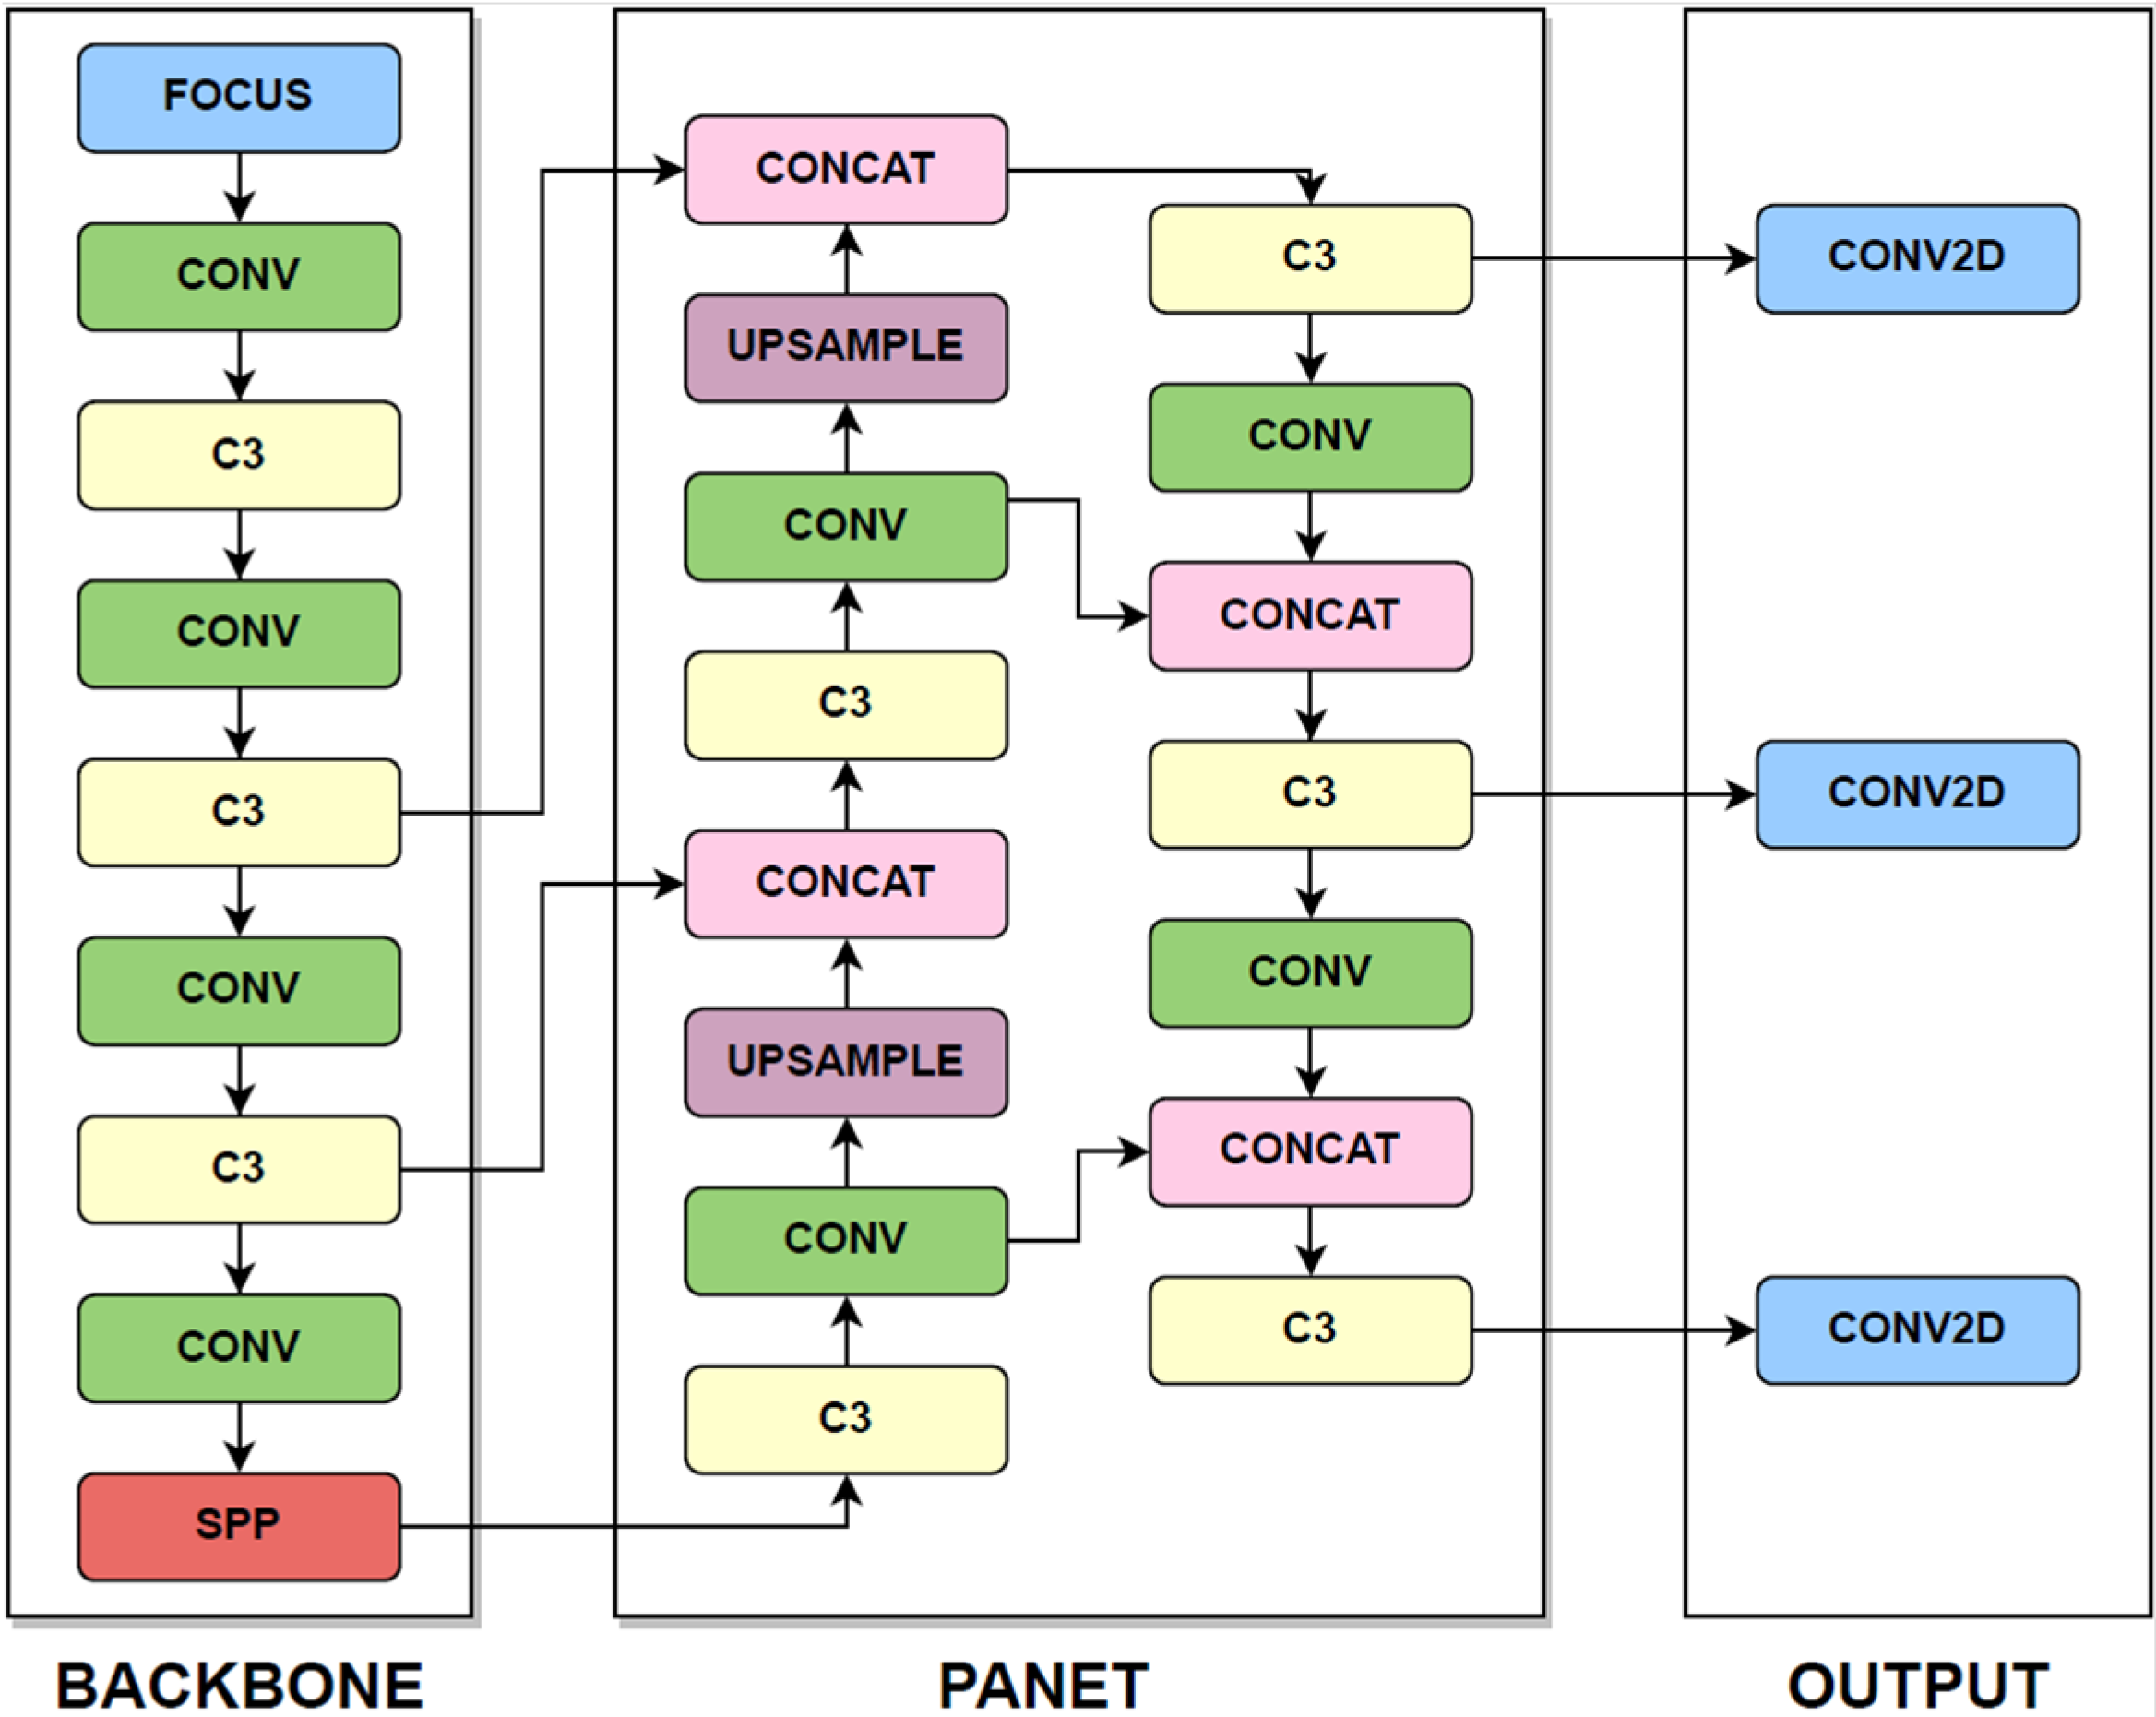
\includegraphics[width=0.65\textwidth]{2/2_teoria/figures/yoloV5.png} % Ajusta el tamaño y ruta
    \caption{Arquitectura de YOLOv5.}
    \label{fig:etiqueta_imagen} % Para referenciar la imagen en el texto
\end{figure}


Finalmente, YOLOv5 es un gran paso adelante en los algoritmos de identificación de objetos, que se aleja de sus predecesores al aprovechar el marco PyTorch e incorporar la red troncal CSPDarknet53 con una nueva arquitectura de agrupación. Esta arquitectura resuelve los problemas de fusión de características y eficiencia computacional, mejorando la precisión de la localización de objetos y reduciendo el tamaño del modelo. La capa de enfoque mejora el uso de la memoria y la eficiencia de propagación.

\subsection{HOG}
El histograma de gradientes orientados (HOG) es un descriptor de características como el detector de bordes de Canny y la transformación de características e invariantes de escala (SIFT). Se utiliza en la visión artificial y el procesamiento de imágenes con el fin de detectar objetos. La técnica cuenta las ocurrencias de orientación de gradiente en la parte localizada de una imagen.

\subsubsection{Prepare la imagen de entrada}
Tome la entrada de la imagen que desea calcular las características HOG. Para ello se tiene que renderizar el tamaño de la imagen a una imagen de 128x64 píxeles (128 píxeles de alto y 64 píxeles de ancho).
\begin{figure}[H]
    \centering
    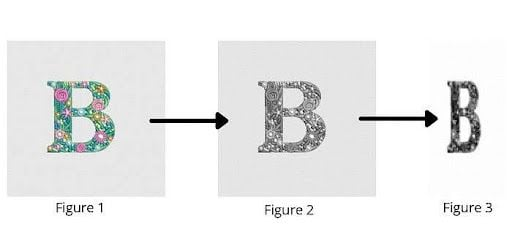
\includegraphics[width=0.60\textwidth]{2/2_teoria/figures/Hog1.jpeg} % Ajusta el tamaño y ruta
    \caption{Preprocesamiento de la imagen.}
    \label{fig:etiqueta_imagen} % Para referenciar la imagen en el texto
\end{figure}

\subsubsection{Calcula el Degradado de la Imagen}
Para calcular el degradado de la imagen debemos conocer que esta compuesto en dos parte gradientes y magnitud.

El gradiente se obtiene combinando la magnitud y el ángulo de la imagen. Considere un bloque de 3x3 píxeles, primero se calcula Gx y Gy para cada píxel utilizando la siguiente fórmula para cada valor de píxel.

\[
G_x(r,c) = I(r,c+1) - I(r,c-1) \quad G_y(r,c) = I(r-1,c) - I(r+1,c)
\]


Después de calcular Gx y Gy, la magnitud y el ángulo de cada píxel se calculan utilizando la fórmula que se menciona a continuación.

\[
\text{Magnitude}(\mu) = \sqrt{G_x^2 + G_y^2} \quad \text{Angle}(\theta) = \left| \tan^{-1}\left(\frac{G_y}{G_x}\right) \right|
\]

\begin{figure}[H]
    \centering
    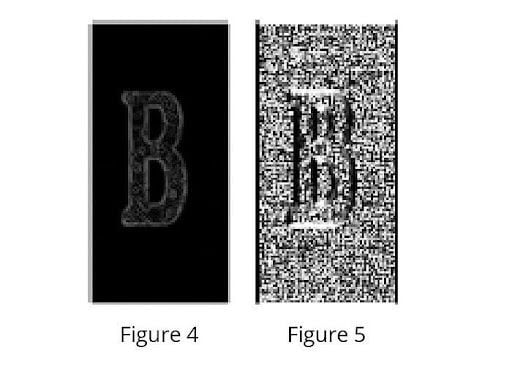
\includegraphics[width=0.55\textwidth]{2/2_teoria/figures/Hog2.jpeg} % Ajusta el tamaño y ruta
    \caption{Degradado de la imagen.}
    \label{fig:etiqueta_imagen} % Para referenciar la imagen en el texto
\end{figure}

\subsubsection{Divide las matrices de degradado para formar un bloque}
Después de obtener el gradiente de cada píxel, las matrices de gradiente (matriz de magnitud y ángulo) se dividen en celdas de 8x8 para formar un bloque. Para cada bloque, se calcula un histograma de nueve puntos. Un histograma de nueve puntos desarrolla un histograma con nueve bins y cada bin tiene un rango de ángulo de 20 grados.
\begin{figure}[H]
    \centering
    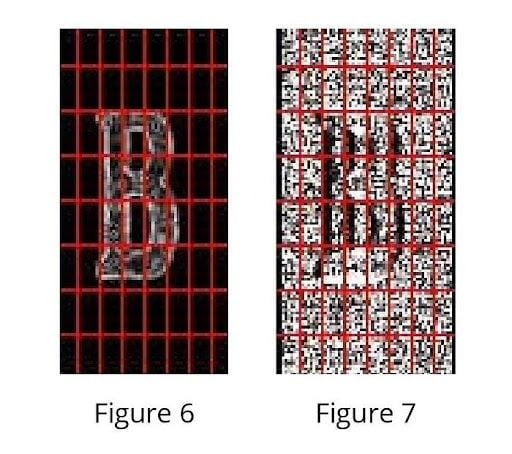
\includegraphics[width=0.55\textwidth]{2/2_teoria/figures/Hog3.jpeg} % Ajusta el tamaño y ruta
    \caption{División de Matrices en bloques.}
    \label{fig:etiqueta_imagen} % Para referenciar la imagen en el texto
\end{figure}

\subsubsection{Agrupar los bloques}
Una vez finalizado el cálculo del histograma para todos los bloques, cuatro bloques de la matriz del histograma de nueve puntos se agrupan para formar un nuevo bloque (2x2). Este aporreado se realiza de forma superpuesta con un paso de ocho píxeles. Para las cuatro celdas de un bloque, concatenamos todos los histogramas de nueve puntos para cada celda constituyente para formar un vector de 36 características.

\begin{figure}[H]
    \centering
    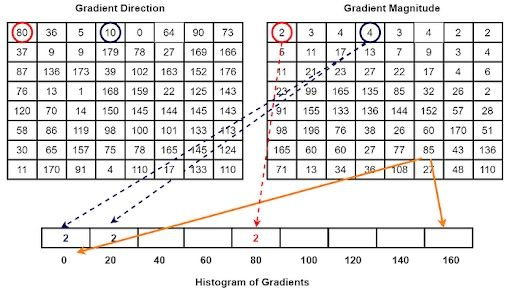
\includegraphics[width=0.50\textwidth]{2/2_teoria/figures/Hog4.jpg} % Ajusta el tamaño y ruta
    \caption{Calculo de Histograma.}
    \label{fig:etiqueta_imagen} % Para referenciar la imagen en el texto
\end{figure}

\subsubsection{Normalizar el valor }
Esta normalización se realiza para reducir el efecto de los cambios en el contraste entre imágenes del mismo objeto. Para normalizar, el valor de k se calcula primero mediante la siguiente fórmula:

\[
k = \sqrt{b_1^2 + b_2^2 + b_3^2 + \dots + b_{36}^2}
\]
\[
f_{bi} = \left[ \left(\frac{b_1}{k}\right), \left(\frac{b_2}{k}\right), \left(\frac{b_3}{k}\right), \dots, \left(\frac{b_{36}}{k}\right) \right]
\]


\subsubsection{Obtenga las características de HOG}
De cada bloque, se recopila un vector de características de 36 puntos. En la dirección horizontal hay 7 bloques y en la dirección vertical hay 15 bloques. Por lo tanto, la longitud total de las características HOG será: 7 x 15 x 36 = 3780. Se obtienen las características HOG de la imagen seleccionada.

\begin{figure}[H]
    \centering
    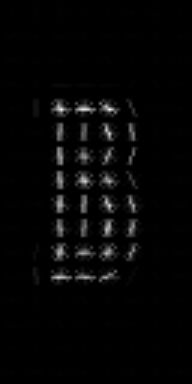
\includegraphics[width=0.20\textwidth]{2/2_teoria/figures/Hog5.jpg} % Ajusta el tamaño y ruta
    \caption{Visualización de características HOG.}
    \label{fig:etiqueta_imagen} % Para referenciar la imagen en el texto
\end{figure}

Por lo tanto, El Histograma de Gradientes Orientados (HoG) se presenta como una técnica robusta y eficiente para la detección de personas, destacándose en entornos dinámicos como las tiendas retail. Su capacidad para identificar siluetas humanas al analizar patrones de gradientes locales lo convierte en una herramienta fundamental para sistemas de vigilancia y análisis de comportamiento del cliente. Esta información permite optimizar la distribución de productos en función del flujo y las preferencias de los consumidores, mejorando la experiencia de compra. Además, HoG no solo es relevante para la detección de personas, sino que también se posiciona como un elemento clave en la transformación digital de las tiendas, conectando la tecnología con la optimización de recursos y la satisfacción del cliente.

% \subsection{SIFT}
% Es un algoritmo para detectar y describir las caracteristicas locales en las imagenes, fue descubierto por David Lowe en 1999. 
% Es un método propuesto por , en el que a una imagen se le transforma en la información en coordenadas invariantes de escala y rotaciones, posteriormente a la luminosidad.

% \subsubsection{Detector}
% Lo primero es obtener un conjunto de puntos de la imagen, los cuales serán denominados keyponints, segun vaya pasando por las diversas etapas, el número de keypoints se irá reduciendo y quedarán los más importantes para ser usados en la comparación.
% \begin{itemize}
%     \item Función scale-space:
%     Se debe realizar una búsqueda de los keypoints en todas las localizaciones de todas las escalas, para lo cual se usa la función continua L(x,y,) convolucionando la imagen I((x,y) y la gausiana.
%     \item Redes Neuronales Convolucionales (CNN): Las CNN destacan por su capacidad para analizar datos visuales, secuenciales y multimodales. En RS, se han utilizado para recomendaciones basadas en texto, imágenes y señales de audio. Ejemplos como DeepCoNN y MusicCNN han mejorado la personalización, mientras que su integración con estructuras de grafos, como CAGCN, aumenta la escalabilidad. Sin embargo, las CNN tienen limitaciones en su capacidad para manejar secuencias largas.
%     \item Redes Neuronales Recurrentes (RNN): Especializadas en datos secuenciales, las RNN han sido fundamentales para recomendaciones basadas en sesiones, como GRU4Rec. Modelos más avanzados, como SASRec, emplean atención para capturar relaciones a largo plazo, y combinaciones con CNN han profundizado en la comprensión de preferencias. A pesar de sus ventajas, enfrentan problemas como gradientes explosivos o desvanecidos, además de un entrenamiento más lento debido a su naturaleza secuencial.
% \end{itemize}


% \subsubsection{Keypoint Descriptor}
% \subsubsection{Matching}

% La coincidencia de imágenes es un aspecto fundamental de muchos problemas de visión artificial, incluido el reconocimiento de objetos o escenas, la resolución de estructuras 3D a partir de múltiples imágenes, la correspondencia estéreo y el seguimiento de movimiento. 
% Se pueden extraer grandes cantidades de características de imágenes típicas con algoritmos eficientes. Además, las características son muy distintivas, lo que permite que una sola característica coincida correctamente con alta probabilidad con una gran base de datos de características, lo que proporciona una base para el reconocimiento de objetos y escenas.
% El reconocimiento de objetos se realiza mediante la coincidencia en primer lugar de cada punto clave de forma independiente de la base de datos de puntos clave extraídos de imágenes de entrenamiento. Muchas de estas coincidencias iniciales serán incorrectas debido a características ambiguas o características que surgen del desorden de fondo. Por lo tanto, primero se identifican las características del grupo al menos 3 que coinciden en un objeto y lo proponen, ya que estos clústeres tienen una probabilidad mucho mayor de ser correctos que las coincidencias de características individuales. A continuación, se comprueba cada clúster realizando un ajuste geométrico detallado al modelo, y el resultado se utiliza para aceptar o rechazar la interpretación.


% El algoritmo SIFT toma una imagen y la transforma en una colección de vectores de características locales. Cada uno de estos vectores de características es distintivo e invariante a cualquier escala, rotación o traslación de la imagen. Estas características no solo son invariantes a la escala y la rotación, sino que también son robustas con respecto al ruido, la oclusión, algunas formas de distorsión afín y los cambios de iluminación. Las características son relativamente fáciles de extraer y también son robustas a la oclusión parcial.

% Por lo tanto, SIFT es un método para extraer características invariantes distintivas de imágenes que se pueden utilizar para realizar una correspondencia confiable entre diferentes imágenes del mismo objeto o escena. El algoritmo SIFT ha llevado a avances significativos en la visión por computadora debido a su eficiencia computacional y efectividad en el reconocimiento de objetos.


\subsection{Datos no Estructurados y Video de Vigilancia}

El análisis de video como fuente de datos no estructurados presenta retos significativos, pero también oportunidades para mejorar la toma de decisiones en el retail. 

Los datos no estructurados no siguen una plantilla específica y predefinida. Además, no están limitados por un modelo de datos específico y predefinido ya que los datos no estructurados no se limitan a documentos de texto sino que abarcan (entre otros) imágenes, grabaciones audiovisuales, correos electrónicos, chats, registros de llamadas, feeds de redes sociales y registros de audio de los centros de llamadas. Los datos no estructurados no se adhieren a los modelos de datos convencionales. Estas formas de datos suelen ser más difíciles de interpretar, según el informe de Deloitte, pero pueden ofrecer una comprensión más completa y holística del panorama general. 

"Debido a que los datos estructurados son más fáciles de trabajar, las empresas ya han podido hacer mucho con ellos", dijo Mikey Shulman. Según algunas estimaciones de la industria, alrededor del 80 por ciento de los datos del mundo no están estructurados.

Es por ello, que los datos no estructurados requiere el uso de técnicas específicas que a menudo son marcadamente diferentes de las empleadas para otros tipos de datos de alta dimensión.

Históricamente, la gestión y utilización de grandes cantidades de datos no estructurados requería mucha mano de obra. Sin embargo, los avances en los modelos de IA han simplificado estas tareas. El contenido de vídeo, en particular, se ha convertido en una importante fuente de datos, ya que ofrece información sobre las reseñas de productos, los comentarios de los clientes y las quejas de las redes sociales.

Por ello, el uso eficaz de los datos no estructurados es esencial para mejorar la participación de los consumidores y aprovechar las diversas fuentes de datos. Ya que, las capacidades de datos no estructurados permiten a los minoristas predecir el comportamiento de los clientes, negociar contratos con proveedores, analizar a la competencia, detectar fraudes y gestionar promociones hiperpersonalizadas. Estas capacidades mejoran los ingresos, el valor del ciclo de vida del cliente y las ganancias a través de la adquisición programática y la gestión de inventario. Por último, los datos no estructurados también son cruciales para recopilar comentarios sobre los productos, informar sobre los ciclos de desarrollo de productos y proporcionar información sobre la demografía de los clientes. Las empresas de bienes de consumo envasados confían en estos datos para comprender el rendimiento del mercado y obtener otros conocimientos valiosos.

\subsection{Sistemas de Recomendación de Distribución de Productos}

Sistema de recomendación son un tipo de sistema de filtrado de información diseñado para predecir y sugerir elementos o contenido, como productos, películas, música o artículos, en los que un usuario podría estar interesado. Estas predicciones se basan en el comportamiento pasado del usuario, sus preferencias o el comportamiento de usuarios similares (\cite{aggarwal2016}). 
El objetivo principal de cualquier sistema de recomendación es mejorar la experiencia del usuario, aumentar el compromiso y facilitar los procesos de toma de decisiones (\cite{berkovsky2008}). Esto es aplicable en varios ámbitos, como el comercio electrónico, el entretenimiento y las redes sociales. Los sistemas de recomendación desempeñan un papel importante tanto en la investigación teórica (académica) como en las aplicaciones prácticas (industria).

En la industria, los sistema de recomendacion mejora la satisfacción del cliente e impulsa el crecimiento de los ingresos al proporcionar sugerencias personalizadas (\cite{amatriain2016}). Grandes corporaciones como Amazon, Netflix y Spotify integran RS en sus operaciones, contribuyendo significativamente a sus modelos de negocio. Por ejemplo, Amazon informa que el 35\% de sus ingresos proviene de su RS (\cite{mackenzie2013}), mientras que Netflix atribuye ingresos de aproximadamente \$ 33.7 mil millones y su éxito en la retención de clientes significativamente a su RS (\cite{iqbal2024}). Se prevé que el mercado mundial de motores de recomendación, según Precision Reports [12] (\cite{precision2024}), experimente un crecimiento sustancial entre 2023 y 2030, lo que pone de manifiesto su creciente importancia en las estrategias empresariales. Los algoritmos que preservan la privacidad y la mitigación de sesgos también se están convirtiendo en áreas clave de enfoque para los profesionales de la industria.

La investigación o las aplicaciones centradas en la práctica suelen considerar las RS como herramientas esenciales para mejorar la participación de los usuarios, la retención y el crecimiento empresarial (\cite{amatriain2016, melville2010}). Es necesaria la colaboración entre el mundo académico y la industria para abordar tanto los desafíos técnicos como las demandas del mundo real, lo que a su vez mejora la satisfacción del usuario y el valor empresarial. Esta interdependencia pone de relieve la creciente importancia de esas asociaciones.

La importancia del sistema de recomendación ha crecido exponencialmente frente a los grandes datos y los avances en la inteligencia artificial (\cite{adomavicius2005, ricci2022}). A medida que los usuarios interactúan con las plataformas digitales, generan grandes cantidades de datos que pueden aprovecharse para hacer precisos



\subsubsection{Deep Learning en los Sistemas de Recomendación}
En los últimos años, el deep learning se ha consolidado como un estándar en los sistemas de recomendación (RS). Esta evolución ha permitido abordar desafíos complejos, mejorando la precisión y personalización de las recomendaciones gracias a diversas arquitecturas de redes neuronales profundas.

\begin{itemize}
    \item Redes Perceptronas Multicapa (MLP): Tradicionalmente, los RS utilizaban métodos lineales como la factorización matricial, que son limitados para capturar interacciones complejas entre usuarios y elementos. Las MLP, mediante múltiples capas profundas, modelan estas relaciones no lineales, logrando mayor precisión. Sin embargo, presentan desafíos como la complejidad, el riesgo de sobreajuste y problemas de interpretabilidad.
    \item Redes Neuronales Convolucionales (CNN): Las CNN destacan por su capacidad para analizar datos visuales, secuenciales y multimodales. En RS, se han utilizado para recomendaciones basadas en texto, imágenes y señales de audio. Ejemplos como DeepCoNN y MusicCNN han mejorado la personalización, mientras que su integración con estructuras de grafos, como CAGCN, aumenta la escalabilidad. Sin embargo, las CNN tienen limitaciones en su capacidad para manejar secuencias largas.
    \item Redes Neuronales Recurrentes (RNN): Especializadas en datos secuenciales, las RNN han sido fundamentales para recomendaciones basadas en sesiones, como GRU4Rec. Modelos más avanzados, como SASRec, emplean atención para capturar relaciones a largo plazo, y combinaciones con CNN han profundizado en la comprensión de preferencias. A pesar de sus ventajas, enfrentan problemas como gradientes explosivos o desvanecidos, además de un entrenamiento más lento debido a su naturaleza secuencial.
\end{itemize}


El deep learning ha revolucionado los sistemas de recomendación, permitiendo una mejor personalización, escalabilidad y precisión. Sin embargo, enfrenta retos como la complejidad computacional, la interpretabilidad y el manejo de datos secuenciales o ruidosos. La evolución continua de estas tecnologías promete desarrollar sistemas más avanzados y adaptables, beneficiando aún más a diversas industrias como el comercio, entretenimiento y noticias.

% \subsection{Optimización de Flujo de Cliente de un Retail}
% La opotimización de flujo de cliente son combinaciones de estrategias para mejorar la experiencia del cliente generando una experiencia de compra fluida y agradable ya que los productos estan a disposición del cliente evitando aglomeración. Ademas de tener un espacio funcional donde los clientes circulen sin sentirse apretados contribuyendo al ambiente general del retail.
% Las tecnologías de visión por computadora han permitido a los minoristas realizar análisis detallados del movimiento y comportamiento de los clientes, lo cual es esencial para gestionar el flujo de manera efectiva (Labeller et al., 2020; Yenra, 2020).

% La implementación de cámaras de vigilancia inteligentes permite monitorear en tiempo real el tráfico en diferentes áreas de la tienda y, a través de algoritmos de visión por computadora, generar mapas de calor que muestran las zonas de mayor actividad. Estos mapas ayudan a identificar los "puntos calientes" y los "puntos fríos" de la tienda, lo cual proporciona datos críticos para reubicar productos en áreas estratégicas y asegurar que las áreas de alto interés tengan suficiente espacio para el tráfico de clientes (Yenra, 2020). Según Labeller et al. (2020), este tipo de datos es crucial para ajustar la disposición de productos y organizar el diseño del espacio comercial de forma que guíe de manera natural el flujo de personas, evitando las aglomeraciones y optimizando el tiempo que los clientes pasan en cada área.

% \subsection{Métricas de Comportamiento en un Retail}
% La aplicación de visión por computadora y técnicas de inteligencia artificial en el ámbito del retail ha facilitado el análisis de patrones de comportamiento de clientes mediante cámaras de vigilancia y mapas de calor. Estos sistemas de análisis visual permiten detectar áreas de alta afluencia dentro de la tienda, lo que resulta crucial para mejorar la disposición de productos y maximizar el tiempo que los clientes permanecen en las áreas de interés. Los mapas de calor generados muestran las zonas de mayor y menor actividad, proporcionando datos que los minoristas pueden usar para ajustar estrategias de marketing y optimización del diseño de la tienda (Almeida et al., 2020; Lee et al., 2022).

% \subsection{Eficiencia Operativa de un Retail}
% La eficiencia operativa en el sector retail se refiere a la capacidad de optimizar sus recursos, procesos y tiempo de manera que maximice la rentabilidad y el servicio al cliente, minimizando los costos.
% Los sistemas de visión por computadora permiten monitorear el inventario en tiempo real, detectar rápidamente cuándo los productos necesitan reposición y reducir el tiempo de inactividad en la tienda. De acuerdo con Yenra (2020), estos sistemas automatizan tareas como la verificación de inventarios y las alertas de reposición, permitiendo que el personal se enfoque en actividades más estratégicas y de atención directa al cliente. Esta automatización contribuye a reducir costos operativos asociados con la gestión manual de inventarios y disminuye la frecuencia de situaciones de "producto agotado", lo cual es clave para mantener altos niveles de satisfacción del cliente.





 